\chapter{Umsetzung}
Mit der Umsetzung des Konzeptes zeigt sich wie gut dieses Gelungen ist. Nachdem nun geklärt ist, wie die Anwendung aussehen soll und welche Werkzeuge verwendet werden, muss eine Testumgebung aufgebaut werden. Ebenfalls muss der Umgang mit den Frameworks und der \ac{IDE}, zu deutsch integrierte Entwicklungsumgebung, vertraut sein.

\section{Aufbau einer Testumgebung}
\label{sec:integration_ace}
Der Server im Smarthome Lab erledigt rund um die Uhr aufgaben. Dabei überwacht er den Zustand verschiedener Geräte und sorgt dafür das diese erreichbar sind. Auf ihm liegen auch Medien und der Webauftritt, welcher über einen Webserver läuft. Dies muss immer zuverlässig funktionieren. Damit der Betrieb nicht eingeschränkt ist, muss eine virtuelle Testumgebung geschaffen werden. Für diesen Zweck wurde ein Abbild des Servers erzeugt, als alles zuverlässig gearbeitet hat. Auf dem Abbild war neben dem Betriebssystem auch der Webserver mit Webauftritt und die MySQL-Datenbank zu finden. Da diese identisch mit den Daten des Servers waren, konnte realistisch getestet werden. Durch das einfache erstellen von Sicherheitskopien konnte risikofrei Software installiert werden um zu schauen, wie sich diese auf das System auswirkt. Mit den verschieden Sicherheitskopien, konnte bei Problemen immer auf einen alten Stand zurückgegriffen werden.


\begin{figure}[bh]
	\centering
	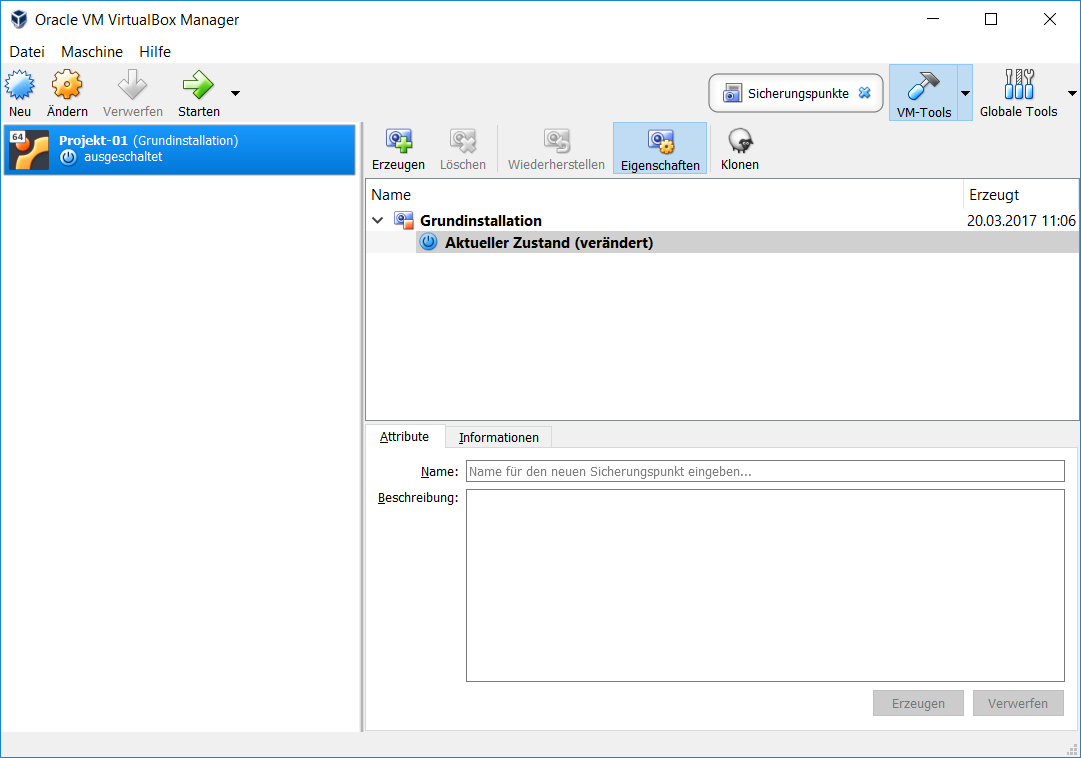
\includegraphics[scale=0.4]{content/pictures/vmware.png}
	% bosch_iot_poll.png: 0x0 pixel, 300dpi, 0.00x0.00 cm, bb=
	\caption{VM-Ware mit geladenem Abbild}
	\label{fig:vmware}
\end{figure}

 In Abbildung \ref{fig:vmware} sieht man den VM-Ware Player. Dieser ist ein kostenloses Tool um Virtuelle Maschinen abzuspielen. Der VM-Ware Player simuliert dabei Hardware, welche im Live-betrieb verändert werden kann. \autocite{vmwareinc.2018} In diesem Fall wird der Server aus dem Smarthome Lab nur Simuliert. Dabei kann ihm mehr speicher hinzugefügt werden, oder auch Seicher entfernt werden. So kam es zu dem Problem, das auf der \ac{VM} nicht ausreichen Festplattenspeicher zur Verfügung stand. In diesem Fall musste die komplette \ac{VM} vergrößert werden. Dies ist mit VM-Ware Player nicht machbar. Unter Windows wird bei der Installation von VM-Ware Player auch der Vdiskmanager installiert. Ein Werkzeug, welches sich über die Kommandozeile steuern lässt. So lässt sich mit dem Befehl \textit{vmware-vdiskmanager -x 100Gb vm.vmdk}, im Verzeichnis der \ac{VM}, die Größe verändern. \autocite{ThomasKrennAG.2018} Damit war ein Vergrößern der \ac{VM} zwar möglich, der zusätzliche Speicher stand zwar physisch, durch eine größere \ac{VM} Datei zur Verfügung, konnte jedoch nicht verwendet werden. In der \ac{VM} wurde ein sogenannter Snapshot verwendet. Bei einem Snapshot, handelt es sich um eine Kopie der \ac{VM} zu einem bestimmten Zeitpunkt. Dieser musste ebenfalls vergrößert werden. Da die Quellen hierzu rar waren, erforderte die Lösung eine lange Suche. Die Lösung ist, mit dem Vdiskmanager den Snapshot auf die gleiche Größe zu bringen. Der Speicher wird nun angezeigt, kann jedoch noch nicht Verwendet werden, da er keiner Partition zugewiesen worden ist. Dies ist über das Betriebssystem, Ubuntu Server 16.04, welches auf der \ac{VM} läuft nicht einfach zu bewerkstelligen. Eine Lösung ist es Ubuntu 18.04 zu verwenden. Dabei wir ein Abbild der DVD, welche für die Installation von Ubuntu benötig wird, in das Virtuelle DVD Laufwerk gelegt. Ubuntu kann ohne Installation verwendet werden. Es liefert das Programm GPartet, mit welchem sich der neue, noch nicht zugewiesene Speicher, der Serverpartition zuweisen lässt. Mit einem Neustart der \ac{VM} und dem Entfernen des Images aus dem virtuellen Laufwerk, hat die \ac{VM} nun ausreichend Festplattenkapazität.\autocite{automatix.}

\subsection{Integration in das Netzwerk}
Da es sich bei der \ac{VM} um ein direktes Abbild des Servers im Smarthome Lab ist, hat es auch die identischen Eigenschaften. So auch die. 

\subsection{MySQL}
Passwort nicht zur verfügung. Neuinstallation notwendig.

\subsection{Nginx}

\section{XAMPP}
Nur für PHP und MySQL lokal 

\section{Austausch von Daten}




\section{Frontend}

\subsection{Commandlineinterface}

\subsection{TypeScript}
Objektorientiert

\subsection{Module}
HTTP

\subsection{Components}

\subsection{Services}





\section{Backend}

\subsection{Composer}

\subsection{Controller}

\subsection{REST}

\subsection{Webserver}


\section{Security}

\subsection{CORS}

\subsection{Token}

\subsection{Salt}


\section{Deploy}
